\documentclass{homework}
\usepackage{homework}
\usepackage{hanhua}
\title{report}
\subtitle{week 9}
\begin{document}

\maketitle
\section{reateTreeOnArray}
\subsection{函数说明}
根据数组建立二叉查找树。
\paragraph{输入}
一个数组指针*nums,一个整型numsSize表示数组大小。
\paragraph{输出}
指向所建立的二叉树根节点的指针。
\paragraph{实现方法}
在输入指针不为空的情况下,依次将数组中数值作为节点插入树中。每次插入过程为:
\begin{enumerate}
    \item 先按照二叉查找树左小右大的规则从根节点旅行到待插入节点的父亲,
    \item 用malloc分配一个节点位置并将父亲对应的指针指向新节点,
    \item 更新新节点的值val和两个子指针(NULL)。
\end{enumerate}
为避免重复节点的出现,用一个HASH数组来确保待插入节点未出现过,并且在插入后更新HASH表。
\subsection{复杂度}
\paragraph{时间复杂度}
平均期望为$\mathcal{O}(n\mathrm{log}n) ~ n$为数组长度。

最坏情况为$\mathcal{O}(n^2)$,如果输入数组为顺序的。因为无法在节点中记录更多信息(如红/黑颜色、平衡度、权重、父亲节点等),不便进行各种平衡树的操作。
\paragraph{空间复杂度}
$\mathcal{O}(n+m)~$n为新建的树占用空间,m为HASH表空间,在本题即数据范围。
\subsection{边界情况}
\begin{itemize}
    \item 传入空指针将得到NULL;
\end{itemize}
\subsection{程序运行结果}
(见下一个函数)
\section{printTree}
\subsection{函数说明}
将二叉树以符合人类阅读习惯的格式打印出来
\paragraph{输入}
指向二叉树根节点的指针*root。
\paragraph{输出}
无返回值,直接将打印结果输出到屏幕。
\paragraph{实现方法}
\begin{enumerate}
    \item 构造一个字符位图,用以记录要打印的内容。(若打印横过来着的树则无需此步骤,访问到节点当场直接打印即可,此举仅为打印正着的树。)
    \item 用中序遍历递归地访问每一个节点,用static变量D记录其深度,将待打印内容储存在字符位图中对应的位置。
    \item 再次返回顶层时代表遍历结束,将整个位图打印出来。
\end{enumerate}
\subsection{复杂度}
\paragraph{时间复杂度}
$\mathcal{O}(n+DW)=\mathcal{O}(DW)~$遍历时间和打印时间。D、W为画树区域的深度和宽度,显然大于节点数n。
\paragraph{空间复杂度}
$\mathcal{O}(n+DW)=\mathcal{O}(DW)~$储存每层是其父的左/右孩子(n)和打印位图(DW)。

而若直接打印竖着的树则空间复杂度为$\mathcal{O}(1)$,若考虑递归过程中系统自己堆栈的话就是$\mathcal{O}(n)$
\subsection{边界情况}
\begin{itemize}
    \item 若有输入的指针为NULL,则打印null;
    \item 打印宽度W为节点数$n\times 2\leqslant 40<80$,高度即为树高$D\leqslant 20$(树退化为链),故$\mathcal{O}(DW)=\mathcal{O}(n^2)$,平均期望为$\mathcal{O}(n\mathrm{log}(n))$;
    \item 由于数据范围较小,将画布大小设为定值,故实际上空间复杂度为$\mathcal{O}(1)$。而如果放宽数据范围,并且不考虑显示器大小,用动态空间记录打印内容的话,空间复杂度才为如上分析。
\end{itemize}
\subsection{程序运行结果}
输入空指针:
\begin{figure}[H]
    \centering
    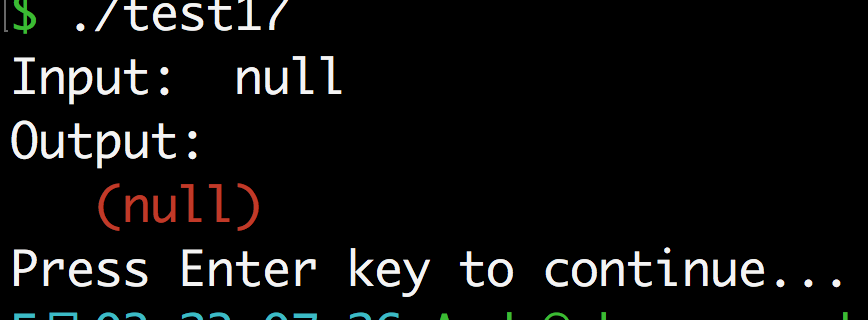
\includegraphics[width=7cm]{null.png}
\end{figure}
若直接打印(横过来的树):
\begin{figure}[H]
    \centering
    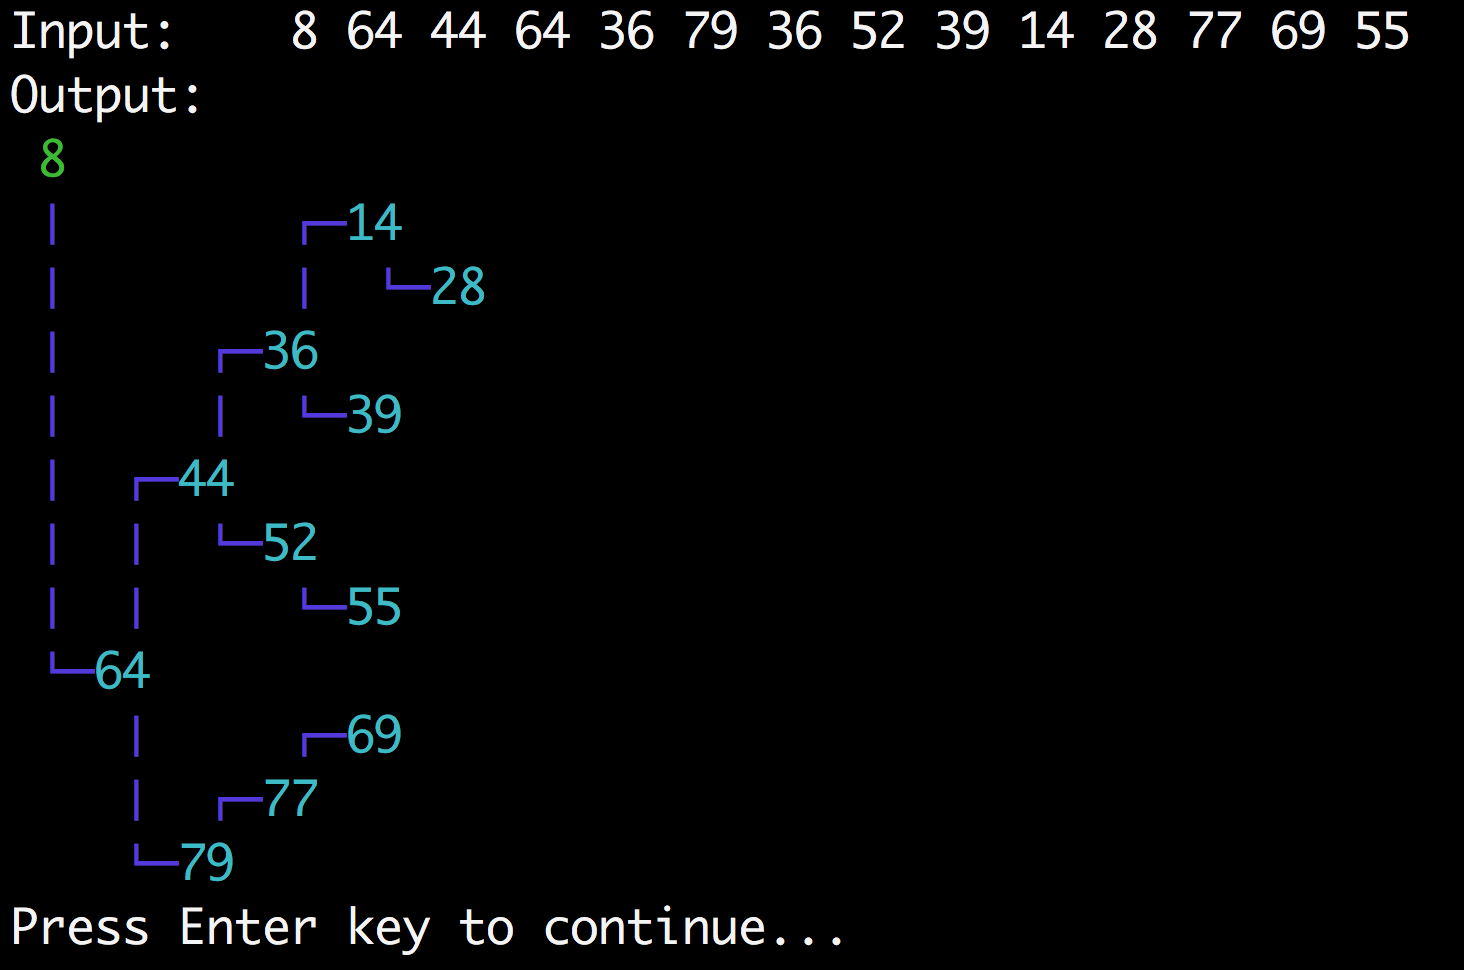
\includegraphics[width=0.8\linewidth]{vert.png}
\end{figure}
最终正着的树打印效果:
\begin{figure}[H]
    \centering
    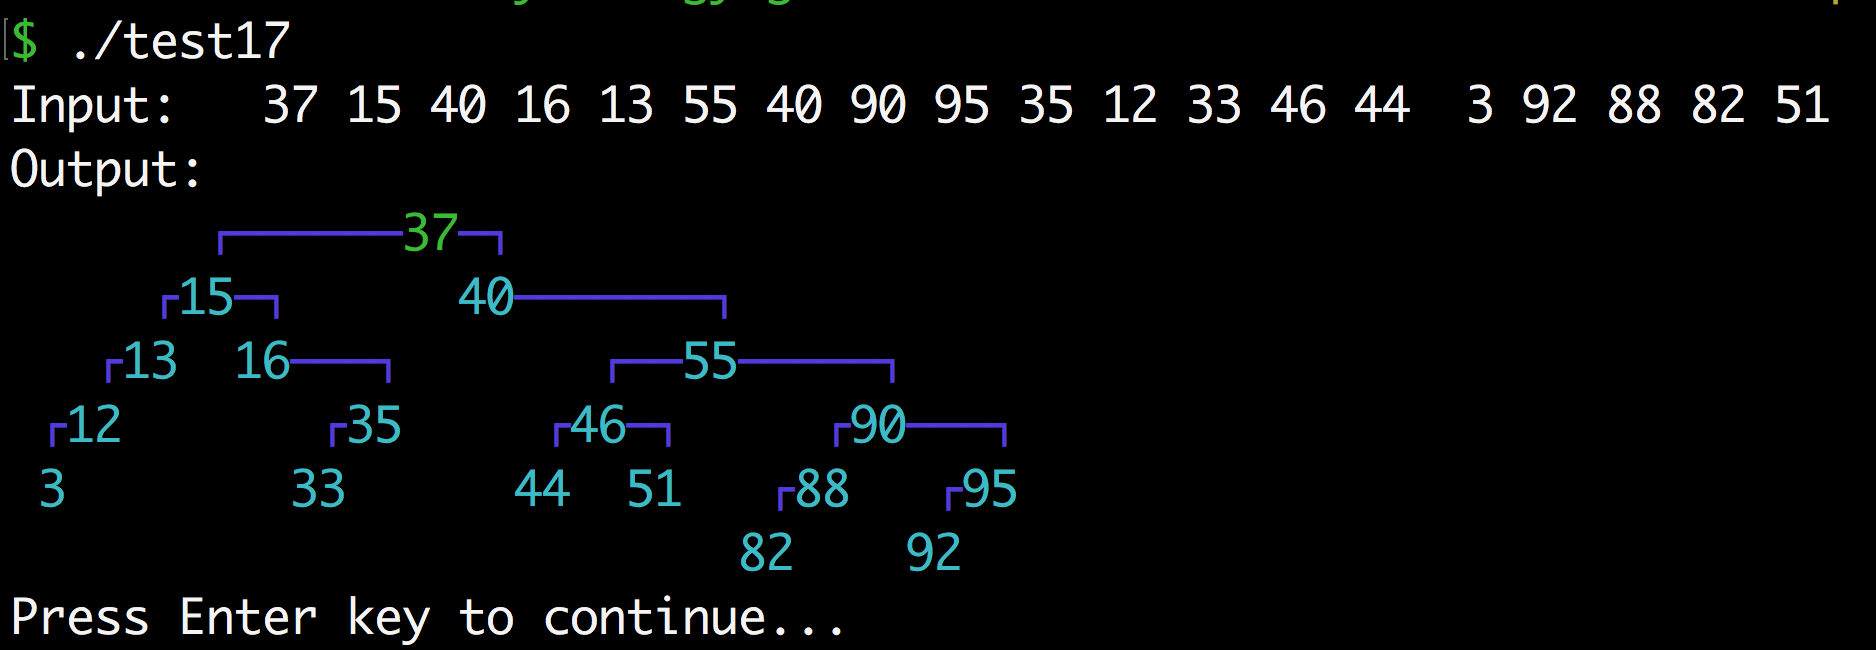
\includegraphics[width=\linewidth]{horz.png}
\end{figure}
\end{document}
